\section{Développement de l'application}

L'application finale demandée reprend les éléments de configuration vus en section 2.
Cette section comporte un récapitulatif des éléments de l'application avec éventuellement des portions de code montrant leur utilisation.
Un exemple de résultats obtenus après lancement de l'application sont montrés.

\subsection{Cahier des charges}

Il s'agit d'implanter une application simple permettant de mesurer le temps de réaction d'une personne (Utilisateur) et mettant en œuvre différentes entrées/sorties disponibles sur la carte SAMD21 en utilisant SW0 et LED0 et sur la carte OLED1 (extension de la carte SAMD21) en utilisant BP1, BP2, BP3, LED1, LED2, LED3 et l'écran OLED.
La structure fonctionnelle de l'application à développer peut être présentée dans un premier temps (légèrement modifiée par la suite) par la figure suivante :

\begin{figure}[h]
    \centering
    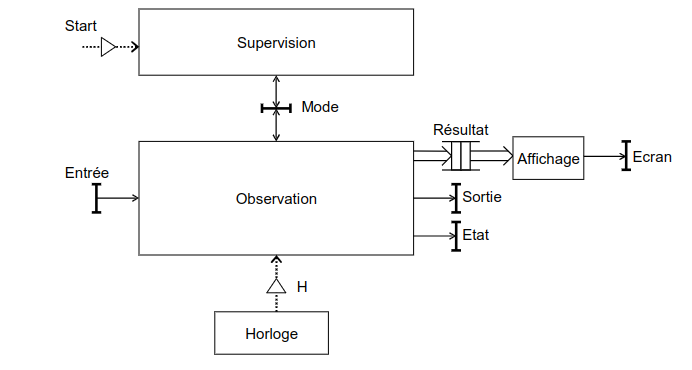
\includegraphics[width=0.7\linewidth]{struct_fonc.png}
    \caption{Structure fonctionnelle initiale de l'application à développer}
    \label{fig:struct}
\end{figure}

La mesure de vitesse de réaction est démarrée lors de l'apparition de l'événement Start.
Elle consiste alors à émettre un code aléatoire en allumant un ensemble de LED (variable Sortie matérialisée par LED1, LED2 et LED3) et à mesurer le temps nécessaire à l'utilisateur pour reproduire la combinaison sur des boutons poussoirs (variable Entrée, matérialisée par BP1, BP2 et BP3) en comptant le nombre d'événements H entre la production d'une valeur sur Sortie et la reproduction de cette valeur sur Entrée. 
Plusieurs mesures de vitesse de réaction peuvent être effectuées afin d'obtenir des valeurs minimale, moyenne et maximale (constante NbMesToDo dans l'automate présenté par la suite, constante dont la valeur est strictement supérieure à 1, peut avoir la valeur 5 par exemple).
Lorsque toutes les mesures ont été effectuées, des statistiques sont transmises à la fonction Affichage qui se charge de les afficher sur l'Ecran de la carte OLED1.
La précision de la mesure du temps de réaction doit être de 1 ms.
L'état de la fonction d'observation (Observe ou Non\_Observe) est en permanence affiché (variable Etat, matérialisée par LED0 de la carte SAMD21XPLAINEDPRO, la LED0 doit être allumée lorsqu'Etat a la valeur Observe).
Le comportement de la fonction Observation est défini par l'automate de la figure 3.


\subsection{Éléments de l'application}

L'application se base sur la structure fonctionnelle suivante :

\begin{figure}[h]
    \centering
    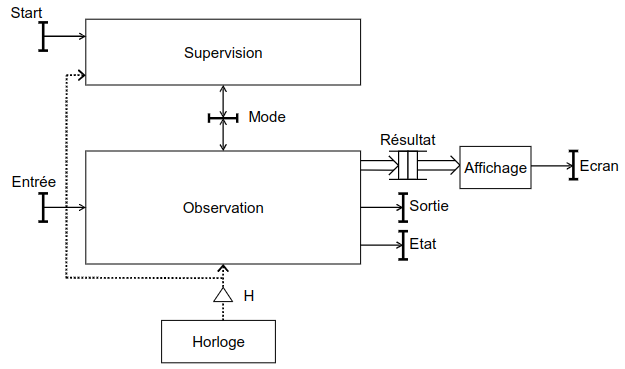
\includegraphics[width=0.7\linewidth]{struct_fonc_final.png}
    \caption{Structure fonctionnelle de l'application à développer}
    \label{fig:struct_final}
\end{figure}

Par rapport à la structure fonctionnelle présentée en figure \ref{fig:struct}, \textit{Start} n'est plus un évènement mais une variable partagée.
Cette solution est plus simple à implanter car elle ne nécessite pas la gestion des interruptions engendrée par l'attente d'un évènement en entrée du système.
De ce schéma, différentes informations peuvent être extraites.
Quatre tâches distinctes peuvent être imaginées pour cette application temps-réel :

\begin{itemize}
    \item Horloge
    \item Supervision
    \item Observation    
    \item Affichage
\end{itemize}

Nous pouvons faire l'hypothèse que deux sémaphores, matérialisées dans la structure par les relations de Start et H, peuvent être implantées au sein de l'application.
L'application contient une variable partagée \textit{Mode} et une file de message \textit{Résultats}.
Les différentes entrées/sorties présentées dans cette structure fonctionnelle correspondent à des éléments physiques présents sur la carte tels que des boutons poussoirs, des LEDs ou l'écran.

\subsection{Résultat}

L'application peut être testée en programmant la carte.
L'utilisateur doit appuyer sur le bouton SW0 pour lancer une série de mesures du temps de réaction.
Dans le cadre des résultats montrés ci-dessous, cinq mesures successives sont effectuées avant l'affichage des résultats sur l'écran.
Les figures suivantes montrent l'affichage de l'écran au lancement de l'application (figure \ref{fig:start_app}) et à la fin d'une série de mesure (figure \ref{fig:end_app}).
Les résultats montrés sont, dans l'ordre:

\begin{itemize}
    \item Le temps de réaction minimal
    \item Le temps de réaction moyen
    \item Le temps de réaction maximal
    \item La période d'observation entre deux appels de la tâche Observation
\end{itemize}

L'unité de chacune de ces valeurs est le \textit{tick d'horloge}.
Le projet utilise une horloge à la fréquence de 8 MHz, divisée par un facteur AAA.
Ainsi, un \textit{tick d'horloge} correspond à approximativement BBB secondes.

\begin{figure}[h]
    \centering
    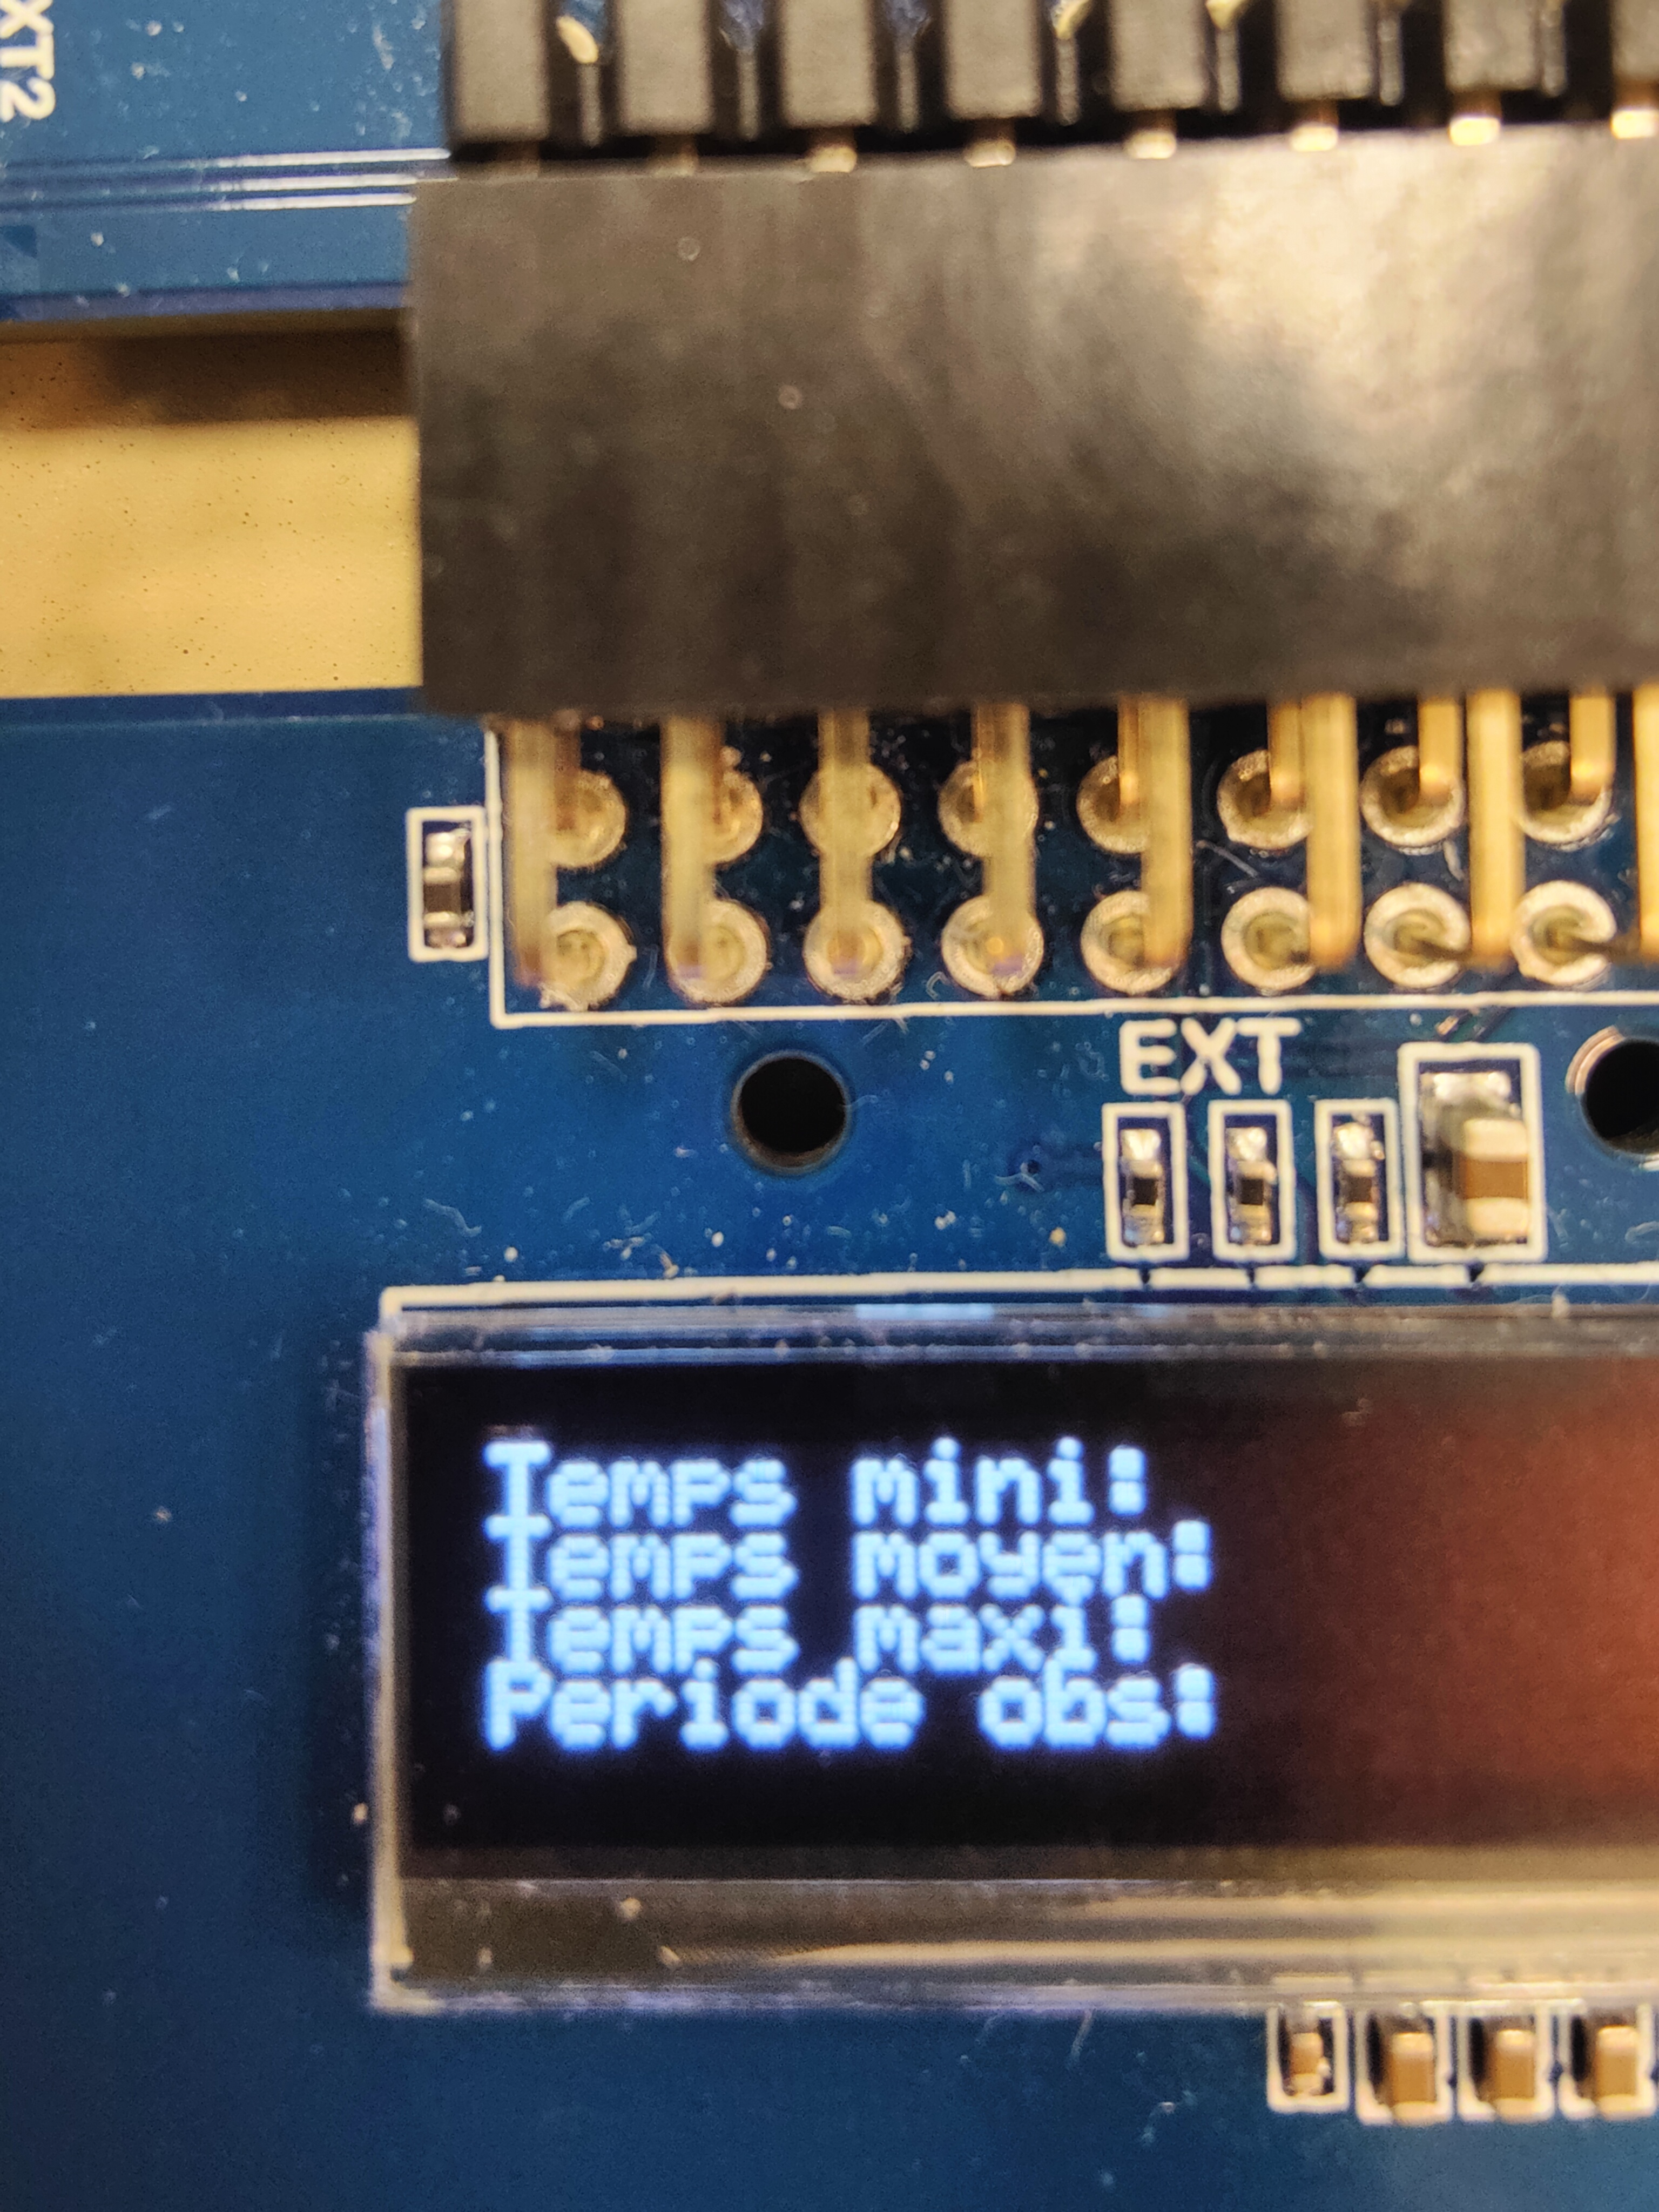
\includegraphics[width=0.4\linewidth]{start_app.jpg}
    \caption{Affichage de l'écran au lancement de l'application}
    \label{fig:start_app}
\end{figure}

Au lancement de l'application, l'écran affiche du texte en préparation de l'arrivée des résultats.
C'est lors de l'initialisation du matériel que cet affichage a lieu.

\begin{figure}[h]
    \centering
    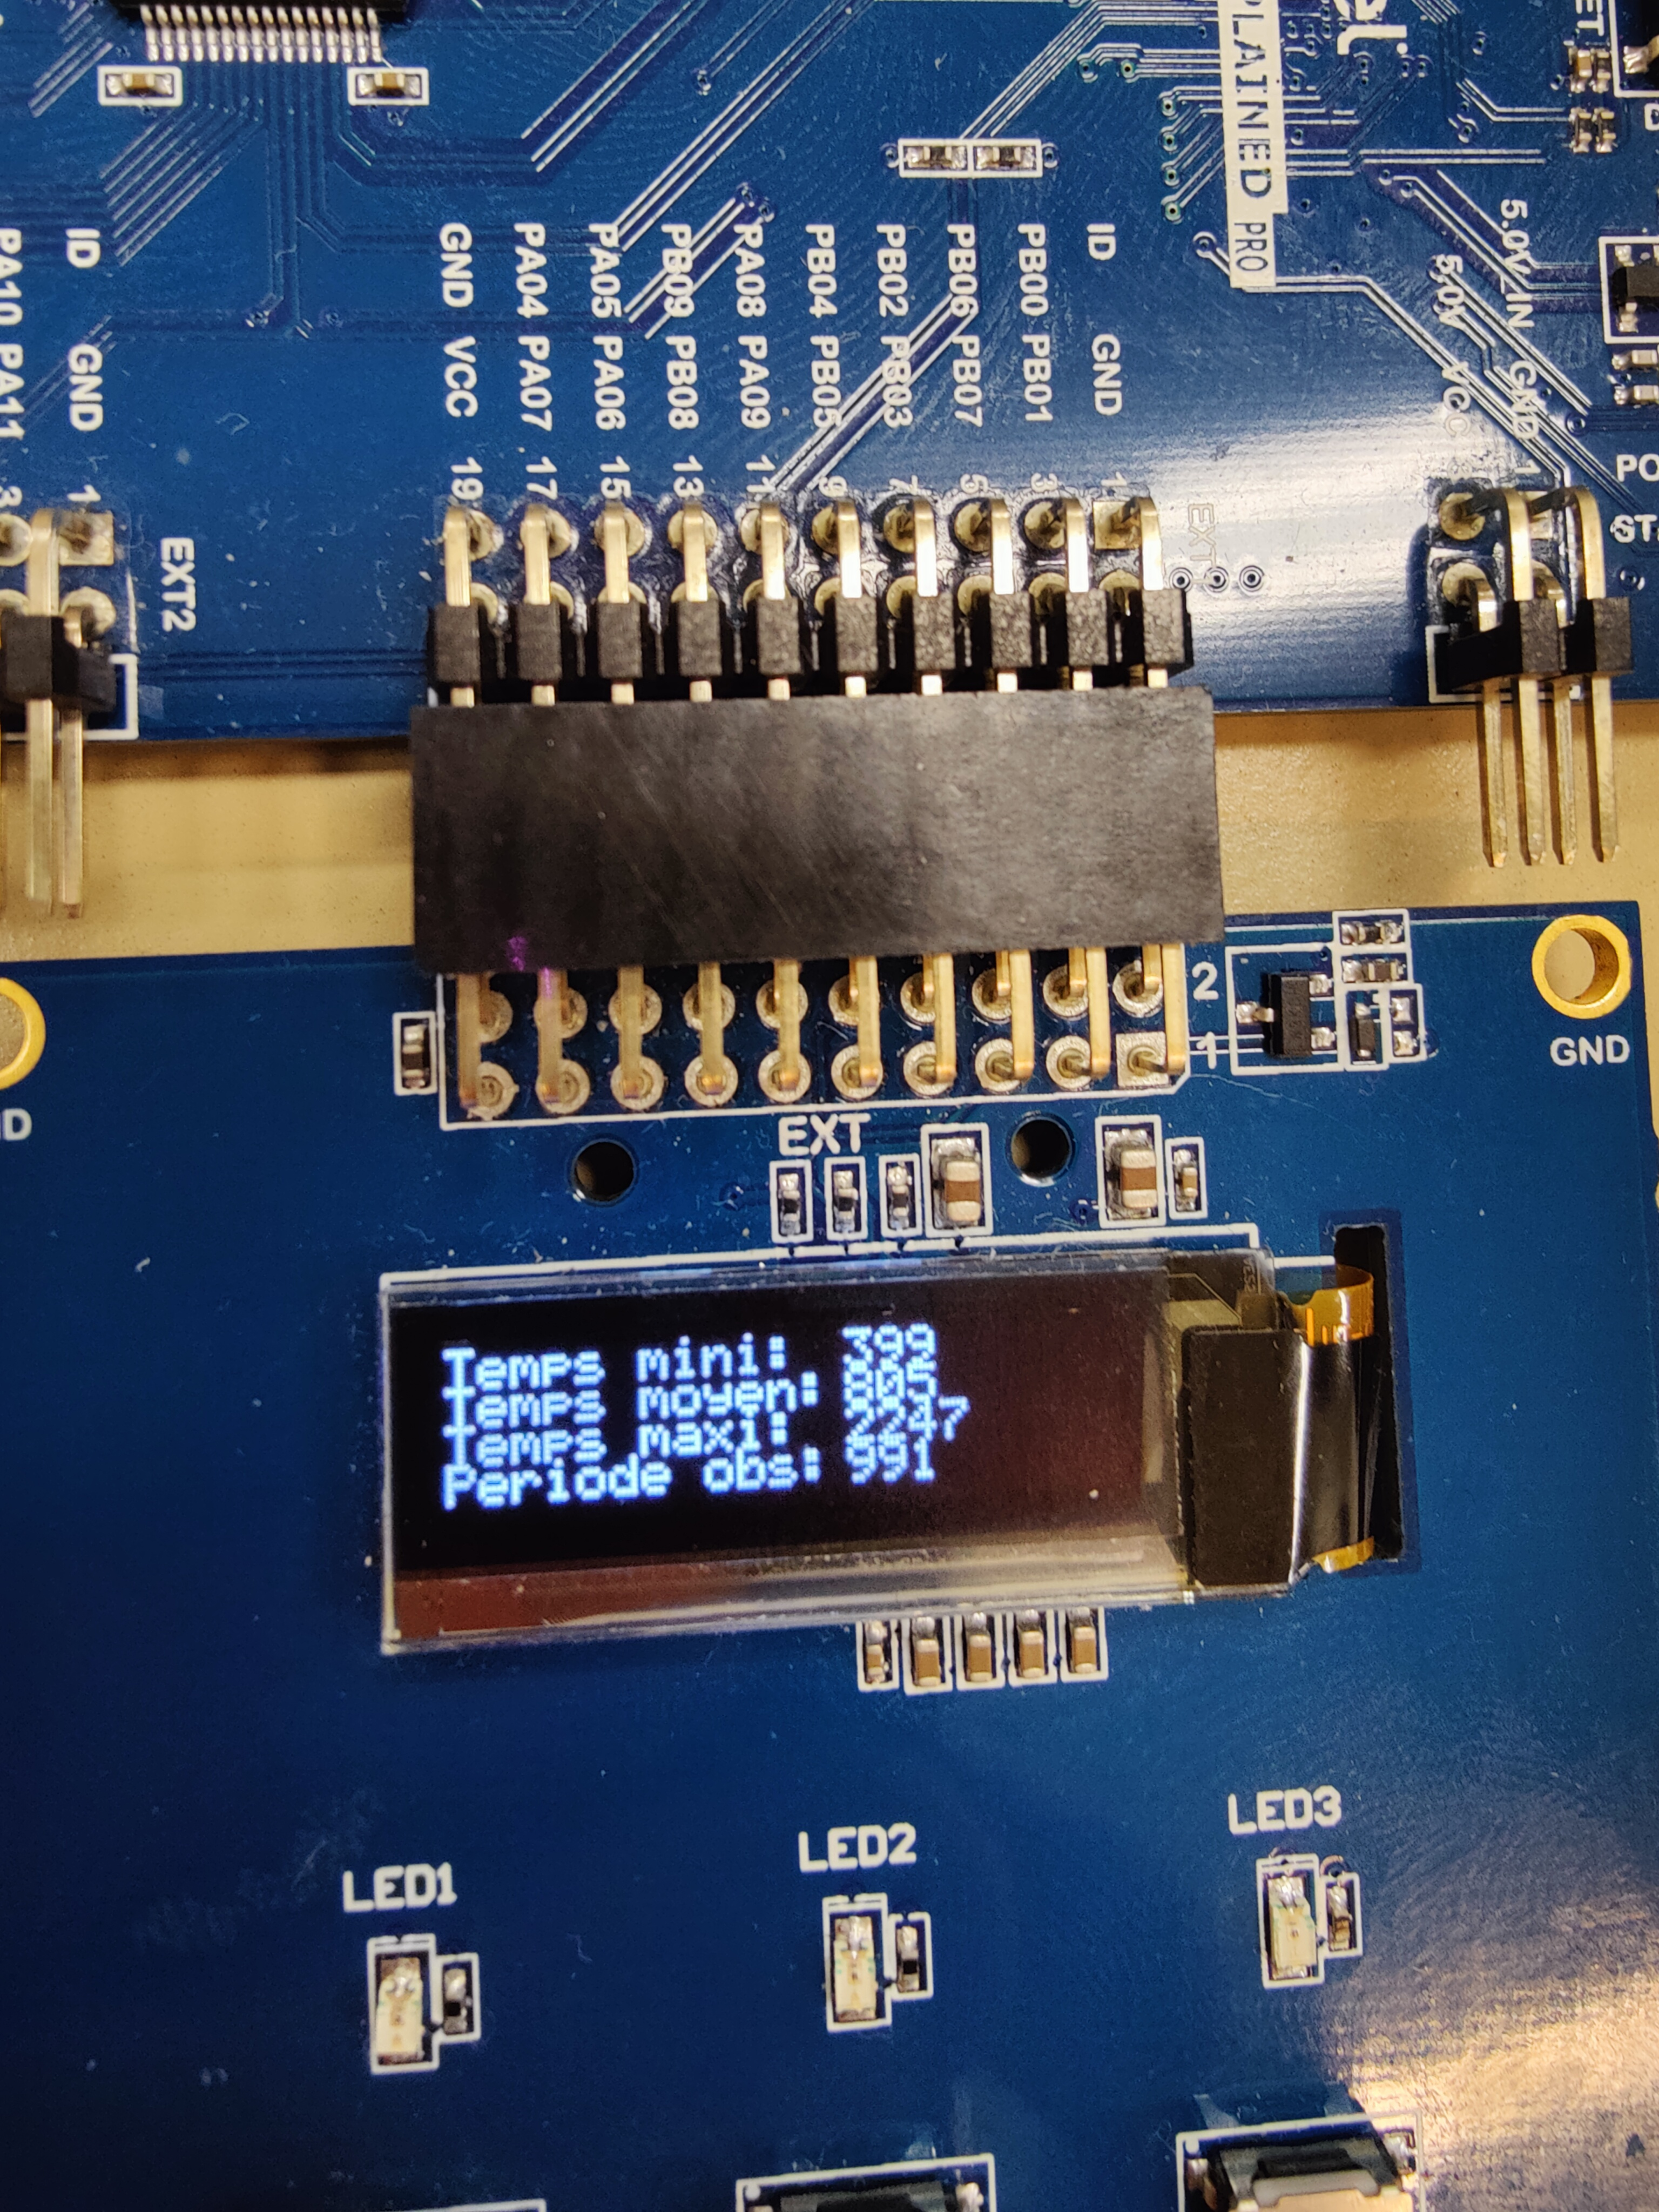
\includegraphics[width=0.4\linewidth]{end_app.jpg}
    \caption{Affichage de l'écran après une session de mesure du temps de réaction}
    \label{fig:end_app}
\end{figure}

Après une série de mesures, la file de message contenant les résultats est envoyée de la tâche \textit{Observation} à la tâche \textit{Affichage}.
Cette file de message contient la variable Résultat, instance de la structure \textit{Resultat\_t} contenant les différentes mesures.
Après réception de la file de message, la tâche \textit{Affichage} fait apparaître sur l'écran les résultats de la mesure.
\\\\
Pour prouver le bon fonctionnement de l'application, une vidéo est proposée dans le même dossier que ce rapport.
Cette vidéo couvre le démarrage de l'application après un reset. 
Une série de mesures a lieu, menant à l'affichage des résultats.
Enfin, l'utilisateur relance une série de mesures après appui sur le bouton SW0.
\\\\
Outre l'aspet fonctionnel de l'application, il est nécessaire de prouver son bon fonctionnement d'un point de vue temps-réel.
La mesure de la période d'obsevation permet de justifier que les tâches s'exécutent dans une fenêtre de temps qui respecte les contraintes temporelles.
La tâche "Observation" est réveillée par une sémaphore en provenance de la tâche "Clock".
Selon la configuration du projet, l'horloge définie par l'OS pour les applications est de 1 khHz.
La tâche "Clock" envoie une sémaphore d'éveil après une attente de 1 Tick d'horloge.
La tâche "Observation" devrait donc être réveillée environ tout les 1000 Ticks d'horloge.
Lors des tests effectués, c'est ce qui a pu être observé, avec une valeur de période d'observation toujours comprise entre 990 et 994.
Dans le cas des résultats présentés en figure \ref{fig:end_app}, la période d'observation est de 991 Ticks d'horloge.